% =====================================================================
% SUPPLEMENTARY NOTE 4 — the six frontier arms.
%
% SOURCES. Benchmark values through table1.collect() (the auditors'
% manifest); per-epoch values from each arm's metrics.csv; prediction
% bands from axw1008/docs/paper/RETRAIN_EXPECTATIONS.md, which was written
% before any arm started. UMAP coordinates from the pinned 400,000-cell
% index, identical for every arm.
%
% REGISTER PASS, 15 November, per SUPPLEMENTARY_REGISTER.md.
% =====================================================================

\section{The six frontier arms}
\label{note:frontier}

The frontier in the main text is traced by six models that differ in two
coefficients and nothing else. In this note we give every model on every
axis, the training record of each, the predictions we specified before any
of them ran, and the latent of each coloured by study. Our purpose is to
let a reader check the two claims the main text makes about the
coefficients: that the adversarial weight moves the achievable trade-off
and then saturates, and that the information cost slides a model along it.

\subsection{The design}

Our two coefficients are $\lambda_{\mathrm{dab}}$, which scales the
reversed gradient from the adversarial study-removal head on its way into
the encoder, and $w_{\mathrm{kl}}$, the weight on the Kullback--Leibler
term that prices the latent (Methods, \emph{Composite objective}). We
arranged them as a three-by-two grid,
$\lambda_{\mathrm{dab}} \in \{7, 168, 336\}$ against
$w_{\mathrm{kl}} \in \{1, 30\}$. Everything else is shared and
byte-identical across the six configuration files, which a test in the
repository enforces: the same vocabulary, the same donor-level split, seed
24, a twenty-epoch horizon with early stopping at a patience of five, and
checkpoint selection by the lowest held-out reconstruction loss. We
adjusted no model after its run started. Each took between 9.1 and 11.2
hours on one A100 (Table~\ref{stab:arms-cost},
Supplementary Fig.~\ref{sfig:hours}), which is the fact behind the main
text's claim that a model of this size can be retrained often enough to
measure a trade-off rather than report a point.

\subsection{Every arm on every axis}

Table~\ref{stab:arms-bio} gives the biological axes and
Table~\ref{stab:arms-cost} the cost axes and the training record.
Table~\ref{stab:arms-p} gives each cross-donor value with its permutation
$P$.

Reading down the $w_{\mathrm{kl}} = 1$ column, raising the adversarial
weight from 7 to 168 moves donor recovery from 0.5837 to 0.5188 and study
separation from 0.8636 to 0.7613, while cross-donor cycle agreement moves
from 0.7337 to 0.7346 and cell family from 0.9829 to 0.9820. Raising it
again to 336 moves donor recovery to 0.5277, study separation to 0.8200 and
the cycle to 0.7146, worse on all three. The $w_{\mathrm{kl}} = 30$ column
repeats that shape: donor recovery 0.5389, 0.3975, 0.4154; study separation
0.8587, 0.6544, 0.7190; cycle 0.6791, 0.6033, 0.5922. In both columns the
middle weight is the best on the cost axes, and 336 gives back part of what
168 bought. That is the saturation the main text describes, and it is why
168 is the weight of both reported models.

Reading across a row, the stronger prior lowers every axis at once. At
$\lambda_{\mathrm{dab}} = 168$ it takes donor recovery from 0.5188 to
0.3975 and study separation from 0.7613 to 0.6544. At the same time it
takes the cycle from 0.7346 to 0.6033, cell family from 0.9820 to 0.9565,
the sixty-way cell type from 0.4964 to 0.4442 and disease from 0.3364 to
0.3045. The same direction holds at 7 and at 336. Thus a coefficient that
moves the cost axes and the biological axes together, in the same
direction, is sliding the model along a trade-off, and a coefficient that
moves the cost axes while the biology holds, and then stops, is moving the
trade-off itself. Overall, the two coefficients behave differently, and the
grid is what shows it.

\begin{table}[p]
\centering
\caption[Every arm, biological axes]{\textbf{The six frontier models and
the five ablations on the biological axes.} Cross-donor excess agreement
for the cycle, cell family, merged severity, rASRM stage and grade; $k$NN
agreement for the sixty-way cell type and for cell-cycle phase; pooled
control-against-eutopic agreement for disease. All on the 416{,}256-cell
held-out split.}
\label{stab:arms-bio}
\footnotesize\setlength{\tabcolsep}{3.5pt}
% GENERATED by figures/scripts/supp_figures.py. Do not edit by hand.
\begin{tabular}{@{}lrrrrrrrr@{}}
\toprule
arm & cycle & family & cell type & cell cycle & disease & severity & stage & grade \\
\midrule
$\lambda_{\mathrm{dab}}$ 7, $w_{\mathrm{kl}}$ 1 & 0.7337 & 0.9829 & 0.5043 & 0.4720 & 0.3449 & 0.1195 & 0.1626 & $-$0.0394 \\
$\lambda_{\mathrm{dab}}$ 7, $w_{\mathrm{kl}}$ 30 & 0.6791 & 0.9841 & 0.4834 & 0.4514 & 0.3483 & 0.1304 & 0.1404 & $-$0.0430 \\
$\lambda_{\mathrm{dab}}$ 168, $w_{\mathrm{kl}}$ 1 & 0.7346 & 0.9820 & 0.4964 & 0.4627 & 0.3364 & 0.1157 & 0.1313 & $-$0.0414 \\
$\lambda_{\mathrm{dab}}$ 168, $w_{\mathrm{kl}}$ 30 & 0.6033 & 0.9565 & 0.4442 & 0.4298 & 0.3045 & 0.1155 & 0.0833 & $-$0.0383 \\
$\lambda_{\mathrm{dab}}$ 336, $w_{\mathrm{kl}}$ 1 & 0.7146 & 0.9779 & 0.4890 & 0.4643 & 0.3558 & 0.0950 & 0.1352 & $-$0.0728 \\
$\lambda_{\mathrm{dab}}$ 336, $w_{\mathrm{kl}}$ 30 & 0.5922 & 0.9553 & 0.4477 & 0.4256 & 0.3304 & 0.1245 & 0.0887 & $-$0.0366 \\
\midrule
random gene grouping & 0.6780 & 0.9606 & 0.4889 & 0.4682 & 0.2698 & 0.0572 & 0.1161 & $-$0.0723 \\
no phase head & 0.4812 & 0.9794 & 0.4536 & 0.4029 & 0.3170 & 0.1429 & 0.1535 & $-$0.0227 \\
no ECS & 0.7397 & 0.9837 & 0.4994 & 0.4681 & 0.3638 & 0.1232 & 0.2190 & $-$0.0438 \\
no DNS sentinel & 0.7308 & 0.9816 & 0.4944 & 0.4729 & 0.3615 & 0.1047 & 0.0799 & $-$0.0549 \\
no order statistics & 0.6384 & 0.9798 & 0.4826 & 0.4622 & 0.3225 & 0.1158 & 0.0918 & $-$0.0358 \\
\bottomrule
\end{tabular}

\end{table}

\begin{table}[p]
\centering
\caption[Every arm, cost axes and training]{\textbf{The cost axes and the
training record.} Donor recovery and study separation are lower-is-better.
val\textsubscript{nb} is the held-out negative-binomial reconstruction loss
at the selected checkpoint; epochs is the number run before early stopping;
best is the selected epoch; hours is wall-clock on one A100.}
\label{stab:arms-cost}
\small
% GENERATED by figures/scripts/supp_figures.py. Do not edit by hand.
\begin{tabular}{@{}lrrrrrr@{}}
\toprule
arm & donor & study sep. & val$_{nb}$ & epochs & best & hours \\
\midrule
$\lambda_{\mathrm{dab}}$ 7, $w_{\mathrm{kl}}$ 1 & 0.5837 & 0.8636 & 0.4016 & 10 & 4 & 10.1 \\
$\lambda_{\mathrm{dab}}$ 7, $w_{\mathrm{kl}}$ 30 & 0.5389 & 0.8587 & 0.4025 & 11 & 5 & 11.2 \\
$\lambda_{\mathrm{dab}}$ 168, $w_{\mathrm{kl}}$ 1 & 0.5188 & 0.7613 & 0.4024 & 10 & 4 & 10.2 \\
$\lambda_{\mathrm{dab}}$ 168, $w_{\mathrm{kl}}$ 30 & 0.3975 & 0.6544 & 0.4046 & 9 & 3 & 9.1 \\
$\lambda_{\mathrm{dab}}$ 336, $w_{\mathrm{kl}}$ 1 & 0.5277 & 0.8200 & 0.3991 & 10 & 4 & 10.2 \\
$\lambda_{\mathrm{dab}}$ 336, $w_{\mathrm{kl}}$ 30 & 0.4154 & 0.7190 & 0.4023 & 9 & 3 & 9.2 \\
\midrule
random gene grouping & 0.5323 & 0.7701 & 0.3911 & 18 & 12 & 18.5 \\
no phase head & 0.3754 & 0.6523 & 0.4083 & 8 & 0 & 8.1 \\
no ECS & 0.5520 & 0.8340 & 0.4004 & 10 & 4 & 8.9 \\
no DNS sentinel & 0.5207 & 0.7818 & 0.4005 & 11 & 5 & 11.1 \\
no order statistics & 0.4943 & 0.7600 & 0.3979 & 10 & 4 & 9.6 \\
\bottomrule
\end{tabular}

\end{table}

\begin{table}[p]
\centering
\caption[Every arm, cross-donor values with $P$]{\textbf{Every cross-donor
value with its permutation $P$}, 200 permutations of the donor-to-label
map, so the floor is 0.005. The cycle and cell family clear their nulls in
every model. Severity among patients and grade clear them in none, and
grade is negative in all eleven.}
\label{stab:arms-p}
\footnotesize\setlength{\tabcolsep}{3pt}
\resizebox{\textwidth}{!}{% GENERATED by figures/scripts/supp_figures.py. Do not edit by hand.
\begin{tabular}{@{}lrrrrrr@{}}
\toprule
arm & cycle & family & severity & patients only & stage & grade \\
\midrule
$\lambda_{\mathrm{dab}}$ 7, $w_{\mathrm{kl}}$ 1 & 0.7337 (0.005) & 0.9829 (0.005) & 0.1195 (0.269) & $-$0.0926 (0.771) & 0.1626 (0.303) & $-$0.0394 (0.492) \\
$\lambda_{\mathrm{dab}}$ 7, $w_{\mathrm{kl}}$ 30 & 0.6791 (0.005) & 0.9841 (0.005) & 0.1304 (0.209) & $-$0.0893 (0.766) & 0.1404 (0.244) & $-$0.0430 (0.512) \\
$\lambda_{\mathrm{dab}}$ 168, $w_{\mathrm{kl}}$ 1 & 0.7346 (0.005) & 0.9820 (0.005) & 0.1157 (0.289) & $-$0.0968 (0.781) & 0.1313 (0.303) & $-$0.0414 (0.497) \\
$\lambda_{\mathrm{dab}}$ 168, $w_{\mathrm{kl}}$ 30 & 0.6033 (0.005) & 0.9565 (0.005) & 0.1155 (0.249) & $-$0.0783 (0.746) & 0.0833 (0.249) & $-$0.0383 (0.527) \\
$\lambda_{\mathrm{dab}}$ 336, $w_{\mathrm{kl}}$ 1 & 0.7146 (0.005) & 0.9779 (0.005) & 0.0950 (0.353) & $-$0.1350 (0.851) & 0.1352 (0.279) & $-$0.0728 (0.667) \\
$\lambda_{\mathrm{dab}}$ 336, $w_{\mathrm{kl}}$ 30 & 0.5922 (0.005) & 0.9553 (0.005) & 0.1245 (0.219) & $-$0.0817 (0.751) & 0.0887 (0.239) & $-$0.0366 (0.517) \\
\midrule
random gene grouping & 0.6780 (0.005) & 0.9606 (0.005) & 0.0572 (0.468) & $-$0.1247 (0.801) & 0.1161 (0.323) & $-$0.0723 (0.627) \\
no phase head & 0.4812 (0.005) & 0.9794 (0.005) & 0.1429 (0.149) & $-$0.0599 (0.766) & 0.1535 (0.119) & $-$0.0227 (0.438) \\
no ECS & 0.7397 (0.005) & 0.9837 (0.005) & 0.1232 (0.274) & $-$0.0978 (0.761) & 0.2190 (0.199) & $-$0.0438 (0.522) \\
no DNS sentinel & 0.7308 (0.005) & 0.9816 (0.005) & 0.1047 (0.333) & $-$0.1137 (0.771) & 0.0799 (0.328) & $-$0.0549 (0.542) \\
no order statistics & 0.6384 (0.005) & 0.9798 (0.005) & 0.1158 (0.279) & $-$0.0785 (0.726) & 0.0918 (0.289) & $-$0.0358 (0.473) \\
\bottomrule
\end{tabular}
}
\end{table}

\begin{figure}[t]
\centering
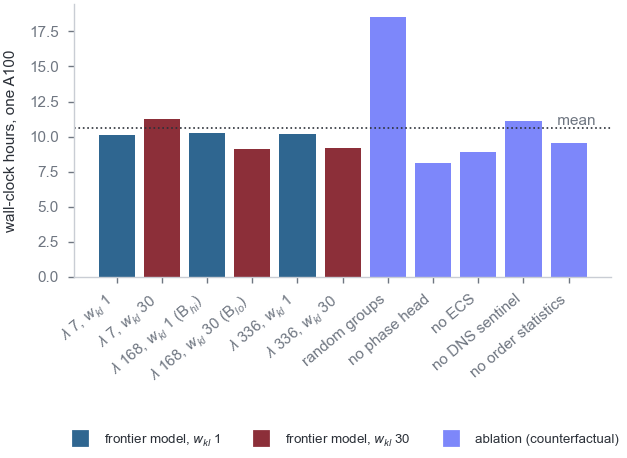
\includegraphics[width=.6\textwidth]{figures/training_hours_all_arms.png}
\caption[Training hours per arm]{\textbf{Wall-clock hours per model on one
A100.} The dotted line is the mean. The longest run is the random-grouping
ablation, which trained for eighteen epochs.}
\label{sfig:hours}
\end{figure}

\subsection{What the training curves show}

Supplementary Fig.~\ref{sfig:loss-p} gives held-out and training
reconstruction loss per epoch for the six models, and
Supplementary Fig.~\ref{sfig:traj-p} the per-epoch validation cycle
agreement. The three $w_{\mathrm{kl}} = 1$ models select epoch 4 and the
three $w_{\mathrm{kl}} = 30$ models epoch 3 or 5, so no selected checkpoint
is a first or a last epoch and every run converged inside the horizon.
Notably, the stronger prior converges one epoch earlier and pays for it in
reconstruction, 0.4046 against 0.4024 at $\lambda_{\mathrm{dab}} = 168$.
In every run the validation cycle agreement rises over the first two to
four epochs and then plateaus, and the selected checkpoints sit on the
plateau.

One caution about that readout. It is $k = 30$ on 19{,}972 validation cells
and is not the benchmark's cross-donor agreement, which is $k = 100$ on the
full held-out split. We use it as a trajectory and not as a value to quote.

\begin{figure}[t]
\centering
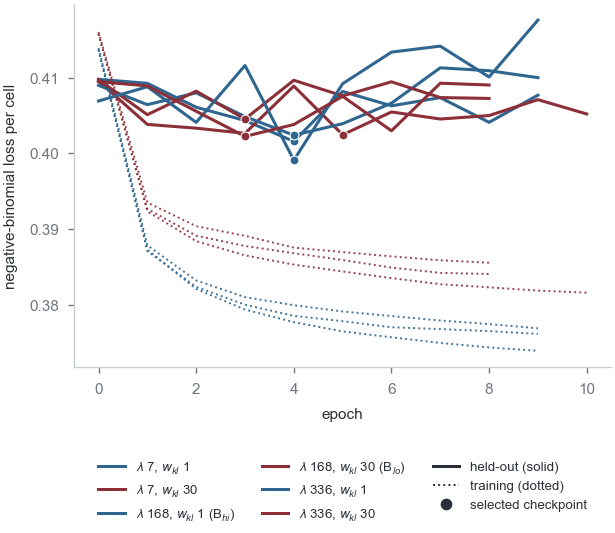
\includegraphics[width=.75\textwidth]{figures/training_loss_pseries.png}
\caption[Reconstruction loss per epoch, frontier arms]{\textbf{Held-out
(solid) and training (dotted) reconstruction loss per epoch for the six
models}, with the selected checkpoint marked. Blue is
$w_{\mathrm{kl}} = 1$, red is 30.}
\label{sfig:loss-p}
\end{figure}

\begin{figure}[t]
\centering
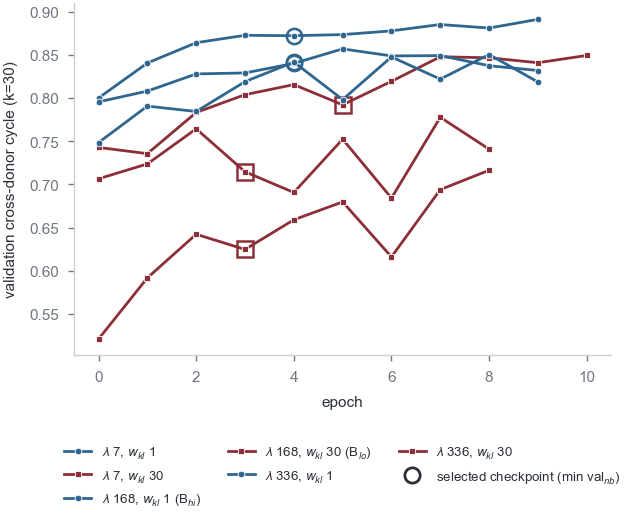
\includegraphics[width=.75\textwidth]{figures/trajectory_cycle_pseries.png}
\caption[Validation cycle agreement per epoch, frontier arms]{\textbf{Validation
cross-donor cycle agreement per epoch}, $k = 30$ on 19{,}972 validation
cells. Open circles mark the selected checkpoint.}
\label{sfig:traj-p}
\end{figure}

\subsection{What was predicted before the runs}

For five of the six models we specified a band for cell family, cycle and
donor recovery before training began, written from the models that preceded
them. The sixth, $\lambda_{\mathrm{dab}} = 336$ at $w_{\mathrm{kl}} = 1$,
was added after the first five had landed and had no band.
Table~\ref{stab:arms-pred} sets each band beside the outcome.

Eight of fifteen landed. Of the seven misses, five are biological axes
landing above their band: the cycle at $w_{\mathrm{kl}} = 30$ in all three
models, 0.6791, 0.6033 and 0.5922 against bands topping out at 0.62, 0.60
and 0.55, the cycle of the reported model at 0.7346 against 0.58 to 0.65,
and cell family at 0.9841 against 0.955 to 0.970. The other two are donor
recovery landing above its band at $w_{\mathrm{kl}} = 30$, 0.5389 against
0.42 to 0.50 and 0.4154 against a ceiling of 0.40. In summary, we
underestimated how much cycle structure survives the strong prior and
overestimated how much donor identity it removes at the weak and the strong
adversary. We keep the bands as written, because an outcome read against a
band written afterwards would be no test at all.

\begin{table}[t]
\centering
\caption[Registered predictions, frontier arms]{\textbf{The bands we
specified before training against the outcomes.} Bands in benchmark terms;
donor recovery is lower-is-better.}
\label{stab:arms-pred}
\small
% GENERATED by figures/scripts/supp_figures.py. Do not edit by hand.
\begin{tabular}{@{}llrrl@{}}
\toprule
arm & axis & registered band & observed &  \\
\midrule
$\lambda_{\mathrm{dab}}$ 7, $w_{\mathrm{kl}}$ 1 & family & $\geq$ 0.965 & 0.9829 & landed \\
$\lambda_{\mathrm{dab}}$ 7, $w_{\mathrm{kl}}$ 1 & cycle & $\geq$ 0.620 & 0.7337 & landed \\
$\lambda_{\mathrm{dab}}$ 7, $w_{\mathrm{kl}}$ 1 & donor & 0.550 to 0.650 & 0.5837 & landed \\
$\lambda_{\mathrm{dab}}$ 168, $w_{\mathrm{kl}}$ 1 & family & $\geq$ 0.960 & 0.9820 & landed \\
$\lambda_{\mathrm{dab}}$ 168, $w_{\mathrm{kl}}$ 1 & cycle & 0.580 to 0.650 & 0.7346 & missed \\
$\lambda_{\mathrm{dab}}$ 168, $w_{\mathrm{kl}}$ 1 & donor & 0.480 to 0.580 & 0.5188 & landed \\
$\lambda_{\mathrm{dab}}$ 7, $w_{\mathrm{kl}}$ 30 & family & 0.955 to 0.970 & 0.9841 & missed \\
$\lambda_{\mathrm{dab}}$ 7, $w_{\mathrm{kl}}$ 30 & cycle & 0.550 to 0.620 & 0.6791 & missed \\
$\lambda_{\mathrm{dab}}$ 7, $w_{\mathrm{kl}}$ 30 & donor & 0.420 to 0.500 & 0.5389 & missed \\
$\lambda_{\mathrm{dab}}$ 336, $w_{\mathrm{kl}}$ 30 & family & 0.940 to 0.960 & 0.9553 & landed \\
$\lambda_{\mathrm{dab}}$ 336, $w_{\mathrm{kl}}$ 30 & cycle & $\leq$ 0.55 & 0.5922 & missed \\
$\lambda_{\mathrm{dab}}$ 336, $w_{\mathrm{kl}}$ 30 & donor & $\leq$ 0.40 & 0.4154 & missed \\
$\lambda_{\mathrm{dab}}$ 168, $w_{\mathrm{kl}}$ 30 & family & 0.955 to 0.967 & 0.9565 & landed \\
$\lambda_{\mathrm{dab}}$ 168, $w_{\mathrm{kl}}$ 30 & cycle & 0.550 to 0.600 & 0.6033 & missed \\
$\lambda_{\mathrm{dab}}$ 168, $w_{\mathrm{kl}}$ 30 & donor & 0.380 to 0.440 & 0.3975 & landed \\
\bottomrule
\end{tabular}

\end{table}

\subsection{The latent of each arm, by study}

Supplementary Figs.~\ref{sfig:umap-7-1} to~\ref{sfig:umap-336-30} give a
two-dimensional UMAP \citep{mcinnes2018umap} of each latent over the same
400{,}000 cells, coloured by study with the eleven-hue palette of Fig.~1.
We pinned the index of those cells to a file so that every model is drawn
on identical cells.

At $\lambda_{\mathrm{dab}} = 7$ the largest study occupies a territory of
its own and several smaller studies sit in lobes with little mixing. At 168
and $w_{\mathrm{kl}} = 1$, the reported B\textsubscript{hi}, the studies
interleave through the central mass and the largest still dominates one
side. At 168 and $w_{\mathrm{kl}} = 30$, B\textsubscript{lo}, the embedding
is a single connected body with studies interleaved throughout. That order
is the order of the study-separation column, 0.8636, 0.7613 and 0.6544, and
the pictures add what the column cannot, which is where in the latent the
remaining separation lives. Supplementary
Fig.~\ref{sfig:umap-base-phase} colours the reported model by menstrual
phase, the structure the stronger prior trades away.

Overall, the six models and their embeddings make one point in two forms.
Pushing the adversary harder buys donor-blindness until it saturates, and
pricing the latent higher buys the same donor-blindness by giving up
biology, so a single correction strength is a position on a trade-off
rather than a description of one.

\begin{figure}[p]\centering
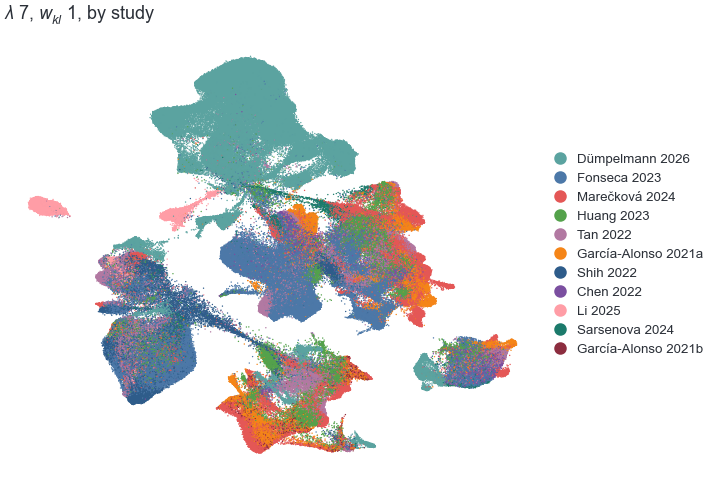
\includegraphics[width=.7\textwidth]{figures/umap_p1_dab7_kl1_study.png}
\caption[UMAP by study, $\lambda_{\mathrm{dab}}$ 7, $w_{\mathrm{kl}}$ 1]{\textbf{UMAP of the
$\lambda_{\mathrm{dab}} = 7$, $w_{\mathrm{kl}} = 1$ latent, by study.}
400{,}000 cells, the same in every panel of this series.}
\label{sfig:umap-7-1}\end{figure}

\begin{figure}[p]\centering
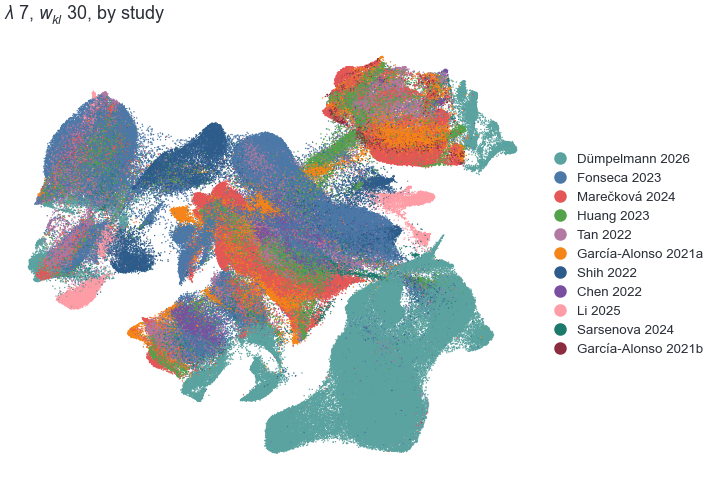
\includegraphics[width=.7\textwidth]{figures/umap_p1_dab7_kl30_study.png}
\caption[UMAP by study, $\lambda_{\mathrm{dab}}$ 7, $w_{\mathrm{kl}}$ 30]{\textbf{UMAP of the
$\lambda_{\mathrm{dab}} = 7$, $w_{\mathrm{kl}} = 30$ latent, by study.}}
\label{sfig:umap-7-30}\end{figure}

\begin{figure}[p]\centering
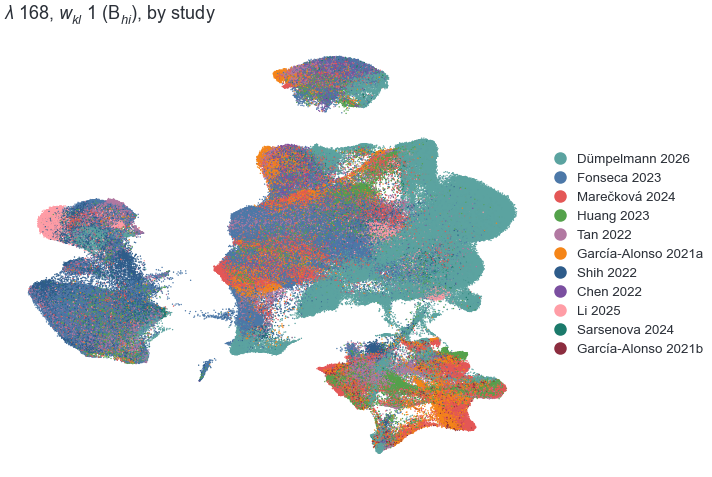
\includegraphics[width=.7\textwidth]{figures/umap_p1_dab168_kl1_study.png}
\caption[UMAP by study, \elaj\,B\textsubscript{hi}]{\textbf{UMAP of the
reported \elaj\,B\textsubscript{hi} latent, by study.}}
\label{sfig:umap-168-1}\end{figure}

\begin{figure}[p]\centering
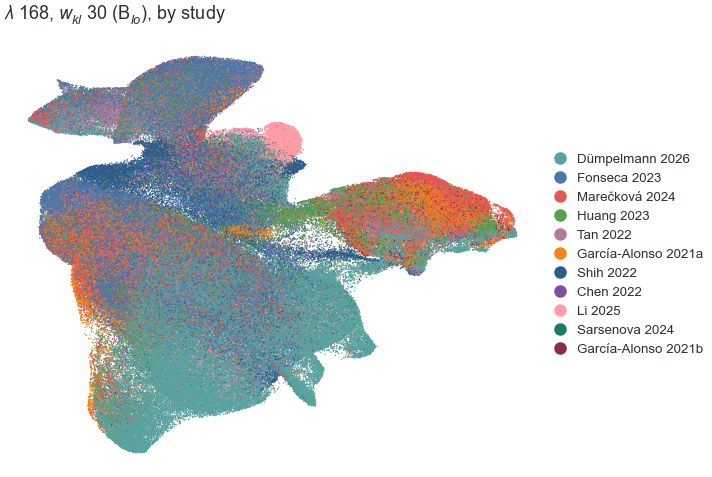
\includegraphics[width=.7\textwidth]{figures/umap_p1_dab168_kl30_study.png}
\caption[UMAP by study, \elaj\,B\textsubscript{lo}]{\textbf{UMAP of the
reported \elaj\,B\textsubscript{lo} latent, by study.}}
\label{sfig:umap-168-30}\end{figure}

\begin{figure}[p]\centering
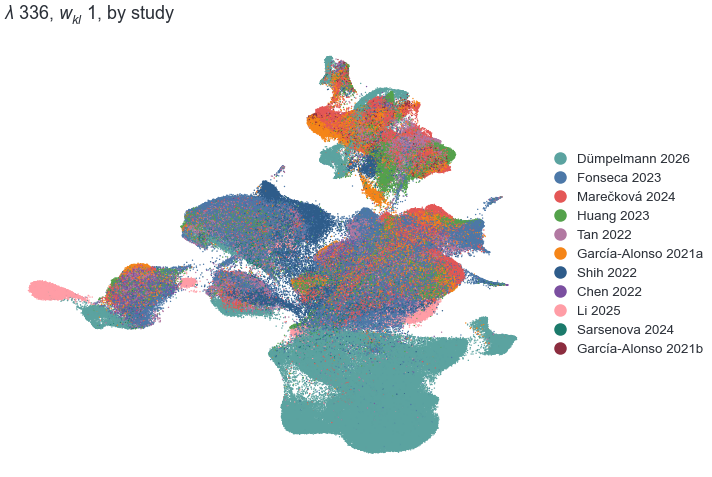
\includegraphics[width=.7\textwidth]{figures/umap_p1_dab336_kl1_study.png}
\caption[UMAP by study, $\lambda_{\mathrm{dab}}$ 336, $w_{\mathrm{kl}}$ 1]{\textbf{UMAP of the
$\lambda_{\mathrm{dab}} = 336$, $w_{\mathrm{kl}} = 1$ latent, by study.}}
\label{sfig:umap-336-1}\end{figure}

\begin{figure}[p]\centering
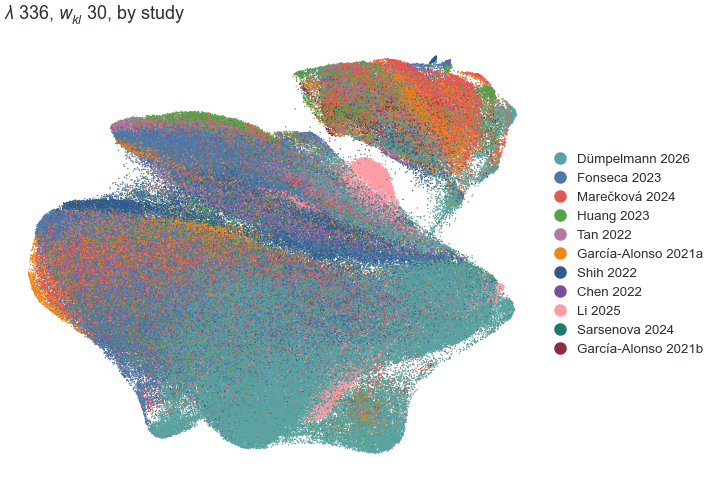
\includegraphics[width=.7\textwidth]{figures/umap_p1_dab336_kl30_study.png}
\caption[UMAP by study, $\lambda_{\mathrm{dab}}$ 336, $w_{\mathrm{kl}}$ 30]{\textbf{UMAP of the
$\lambda_{\mathrm{dab}} = 336$, $w_{\mathrm{kl}} = 30$ latent, by study.}}
\label{sfig:umap-336-30}\end{figure}

\begin{figure}[p]\centering
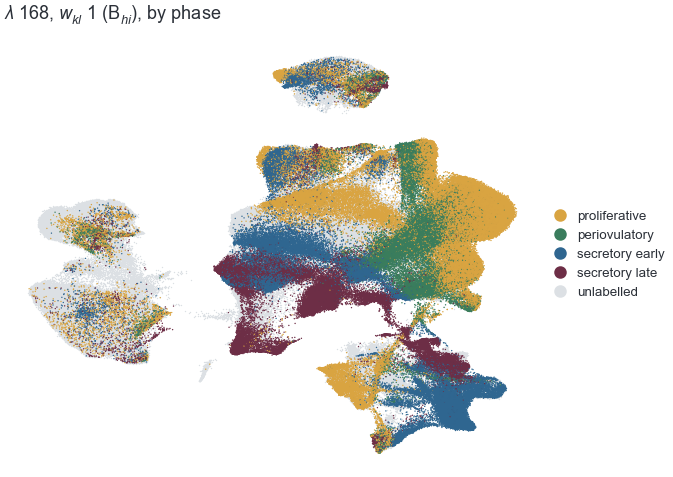
\includegraphics[width=.7\textwidth]{figures/umap_p1_dab168_kl1_phase.png}
\caption[UMAP by phase, \elaj\,B\textsubscript{hi}]{\textbf{The reported
\elaj\,B\textsubscript{hi} latent, by menstrual phase.} Grey cells carry no
phase label.}
\label{sfig:umap-base-phase}\end{figure}
